\section{Social Herding Towards the Median Hypothesis Test}\label{ht}
In this section, we test the \textbf{Social Herding Towards the Median} hypothesis, by analyzing spread of grades around the median grade for the participants that changed their grades.
There are three principle challenges in testing this hypothesis.
The first challenge is that parametric significance tests comparing two sample means such as the two sample t-test and z-test are known to 
perform poorly for multimodal and discrete distributions.
Another significance test that is commonly applied to compare spreads of distributions is the F-test, which is also known to perform poorly for many non-normal distributions \cite{markowski1990conditions}.
Furthermore, this test is usually used to test the spread of data around the mean, which only in very special conditions, such as normal distributions, aligns with the median which is relevant to our problem. 
The discretness of our data leads to mutli-modal distributions which are not optimal for these testing methods.

The second challenge is that there is a natural tendency for grades to concentrate around the median even without a bias.
Consider the following participant behavioral model.
Suppose that participants are not acustomed to a slider-based input.
We can model the first grade that the particpant leaves as uniformly randomly anywhere on the slider.
As the participant begins to understand how to use the slider their use becomes more accurate, ultimately settling on a grade from our observed distribution of final grades.
This model, the first grade is uniformly random and the second grade is a sample from the observed distribution, would result in a strong regression towards the median; even if there is no causal link with seeing the median.

Finally, the median grade $m_i$ can be different for each participant.
The median grade is calculated over all prior participants and thus is dependent on when the participant submitted their first grade.
In practice, the median will eventually converge for a large number of participants, but it would be incorrect to measure concentration around a final median.

To address these three challenges, we propose a non-parametric model based on the Wilcoxon statistic to test the hypothesis that the group of participants that changed their grades are more tightly centered around the median grade that the participants observed.
Our tests compare absolute deviations around the median for $P_n$, $P_c$, and $R$; which, as a relative test, controls for the natural tendency for grades group around the median.
Furthermore, it is more robust to the effects of alternate models such as the one described in our second challenge in comparision to a direct test of correlation.

\subsection{Non-parametric Significance Test}
Recall that $P_n$ is the set of participants that did not change their grades and $P_c$ be the set of participants that changed their grades.
We define a set $X_c,X_n$ of absolute deviations from the observed median of the final grade for each group:
\begin{equation}
X_c = \{|m[j] - g_f[j]|\}\text{ }\forall j \in P_c
\end{equation}
\begin{equation}
X_n = \{|m[j] - g_f[j]|\}\text{ }\forall j \in P_n
\end{equation}
For the purposes of hypothesis testing herding behavior, we ignore the sign of the deviation.
However, in Section \ref{changemod}, where we build a predictive model for the changes, we include the sign.

Now, for the set $X_c$, we calculate the Wilcoxon rank-sum statistic.
We assign a rank to each of the absolute deviations in the union set $\textbf{X} = X_c \cup X_n$ (ie. the largest change has rank 1 and the smallest has rank $|X_c \cup X_n|$.
For $X_c$, we sum the ranks of the deviations within its set:
\begin{equation}
W_c = \sum_{j \in P_c} R_j
\end{equation}

The \textbf{Null Hypothesis} is that absolute deviations in $X_c$ are the same size as $X_n$. 
Under this null hypothesis $median(X_n) = median(X_c)$, the ranks will be evenly distributed between each group. 
Therefore, the null expected value and variance of $W$ is:
\begin{equation}
\mathbb{E}(W) = \frac{(|\textbf{X}| + 1)\cdot |X_c|}{2}
\end{equation}
\begin{equation}
var(W) = \frac{(|\textbf{X}| + 1)\cdot |X_c| \cdot |X_n|}{12}
\end{equation}
For the significance level $\alpha$, we can test the probability that our calcuated $W_c$ comes from the null distribution.
In other words, the test calculates the probability that a random subset of users (ignoring the categorization $P_n$ and $P_c$) can have the observed difference in rank-sum values.
A significant result means that for the participants that changed their grades the changed changes are more tightly centered around the median grade they observed.

The same analysis can be used to test $X_c$ against the absolute deviations in the reference survey $X_r$
\begin{equation}
X_r = \{|m[j] - g_i[j]|\}\text{ }\forall j \in R
\end{equation} 
or for initial vs. final ratings in the change group $X_c'$:
\begin{equation}
X_c' = \{|m[j] - g_i[j]|\}\text{ }\forall j \in P_c
\end{equation}

\subsection{Quantifying Concentration of Grades}
In addition to testing the hypothesis, we can also quantify the effects of social herding. 
We tested the significance of the absolute deviations using a Wilcoxon test statistic.
The Wilcoxon statistic can be inverted to estimate a most likely \emph{shift parameter}, that a constant shift $\Delta$ in the distribution of absolute deviations $X_c$ that maximally aligns them with $X_n$ (ie. $X_c + \Delta$ is most supported by the null hypothesis). 
Since $X_c$ is a set of absoulte deviations, $\Delta$ tells us how much more concentrated $X_c$ is than $X_n$ around the observed medians.
This parameter is relevant to the design of recommendation algorithms use proximity (eg. clustering or nearest neighbors).

We refer to \cite{lehmann2006nonparametrics} on the derivation of $\Delta$ and its confidence interval:
\begin{equation}
D = \{x_n[j] - x_c[i]\} \text{ } \forall i,j \in X_n, X_c
\end{equation}
\begin{equation}
\Delta = median(D)
\end{equation}

%\subsection{Discussion About the Grade Distribution}
%In Figure \ref{dist-1}, we show the distribution of absolute deviations for the Marriage Rights issue. 
%\begin{figure}[ht!]
%  \centering
%    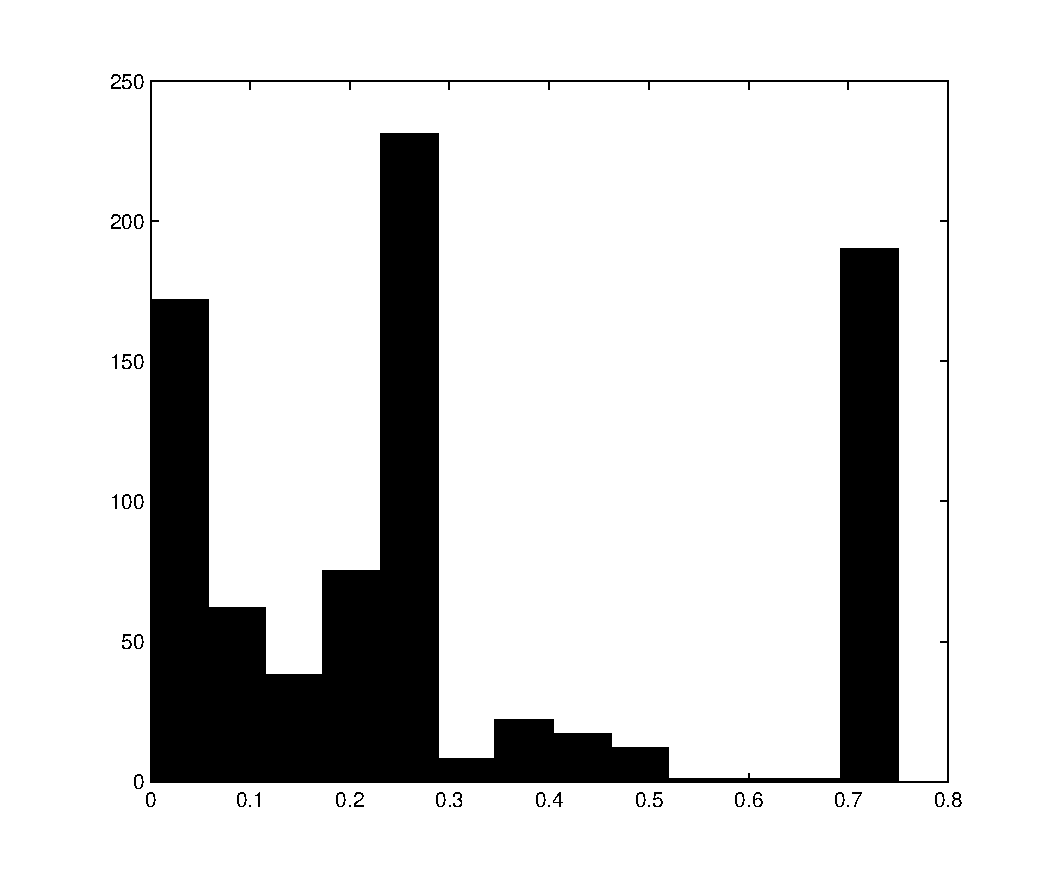
\includegraphics[scale=0.40]{../plots/absolute-deviations.eps}
%      \caption{\textbf{TODO}}
%      \label{dist-1}
%\end{figure}
%We see that the distribution is multimodal and discrete. 
%Parametric tests such as the z-test and the t-test have been shown to have weaker statistical power in many families of multimodal distributions such as mixtures of Gaussians \cite{???}.
%Rank-based tests tend to be more robust to the multimodality and in fact don't depend on the actual values on the relative frequency of the ranks in the test set.



